\documentclass[a4paper, 11pt]{article}
\usepackage{comment} % enables the use of multi-line comments (\ifx \fi) 
\usepackage{lipsum} %This package just generates Lorem Ipsum filler text. 
\usepackage{fullpage} % changes the margin
\usepackage[a4paper, total={7in, 10in}]{geometry}
\usepackage[fleqn]{amsmath}
\usepackage{amssymb,amsthm}  % assumes amsmath package installed
\newtheorem{theorem}{Theorem}
\newtheorem{corollary}{Corollary}
\usepackage{graphicx}
\usepackage{tikz}
\usetikzlibrary{arrows}
\usepackage{verbatim}
\usepackage[numbered]{mcode}
\usepackage{float}
\usepackage{tikz}
    \usetikzlibrary{shapes,arrows}
    \usetikzlibrary{arrows,calc,positioning}

    \tikzset{
        block/.style = {draw, rectangle,
            minimum height=1cm,
            minimum width=1.5cm},
        input/.style = {coordinate,node distance=1cm},
        output/.style = {coordinate,node distance=4cm},
        arrow/.style={draw, -latex,node distance=2cm},
        pinstyle/.style = {pin edge={latex-, black,node distance=2cm}},
        sum/.style = {draw, circle, node distance=1cm},
    }
\usepackage{xcolor}
\usepackage{mdframed}
\usepackage[shortlabels]{enumitem}
\usepackage{indentfirst}
\usepackage{hyperref}
    
\renewcommand{\thesubsection}{\thesection.\alph{subsection}}

\newenvironment{problem}[2][Problem]
    { \begin{mdframed}[backgroundcolor=gray!20] \textbf{#1 #2} \\}
    {  \end{mdframed}}

% Define solution environment
\newenvironment{solution}
    {\textit{Solution:}}
    {}

\renewcommand{\qed}{\quad\qedsymbol}
%%%%%%%%%%%%%%%%%%%%%%%%%%%%%%%%%%%%%%%%%%%%%%%%%%%%%%%%%%%%%%%%%%%%%%%%%%%%%%%%%%%%%%%%%%%%%%%%%%%%%%%%%%%%%%%%%%%%%%%%%%%%%%%%%%%%%%%%
\begin{document}
%Header-Make sure you update this information!!!!
\noindent
%%%%%%%%%%%%%%%%%%%%%%%%%%%%%%%%%%%%%%%%%%%%%%%%%%%%%%%%%%%%%%%%%%%%%%%%%%%%%%%%%%%%%%%%%%%%%%%%%%%%%%%%%%%%%%%%%%%%%%%%%%%%%%%%%%%%%%%%
\large\textbf{Your names: Project Group} \hfill \textbf{Problem Set - 5}   \\
Email: reh161@case.edu \hfill ID: 3451423\\
\normalsize Course: CSDS 337 - Compiler Design \hfill Term: Spring 2023\\
Instructor: Dr. Vipin Chaudhary \hfill Due Date: $17^{th}$ April, 2023 \\ \\
Number of hours delay for this Problem Set: \hfill 0 \\
Cumulative number of hours delay so far: \hfill \\ 69 \\
I discussed this homework with: \hfill \\ \\
%\underline{\bf SUBMISSION GUIDELINES:} Submit a zip file that includes the %written answers and the flex file for Problem 4. \\

\noindent\rule{7in}{2.8pt}
%%%%%%%%%%%%%%%%%%%%%%%%%%%%%%%%%%%%%%%%%%%%%%%%%%%%%%%%%%%%%%%%%%%%%%%%%%%%%%%%%%%%%%%%%%%%%%%%%%%%%%%%%%%%%%%%%%%%%%%%%%%%%%%%%%%%%%%%
% Problem 1
%%%%%%%%%%%%%%%%%%%%%%%%%%%%%%%%%%%%%%%%%%%%%%%%%%%%%%%%%%%%%%%%%%%%%%%%%%%%%%%%%%%%%%%%%%%%%%%%%%%%%%%%%%%%%%%%%%%%%%%%%%%%%%%%%%%%%%%%

%%%%%%%%%%%%%%%%%%%%%%%%%%%%%%%%%%%%%%%%%%%%%%%%%%%%%%%%%%%%%%%%%%%%%%%%%%%%%%%%%%%%%%%%%%%%%%%%%%%%%%%%%%%%%%%%%%%%%%%%%%%%%%%%%%%%%%%%


\begin{problem}{1 - 10 points}
The C code to compute Fibonacci numbers recursively is shown below. Suppose that the activation record for $f$ includes the following elements  in order: (return value, argument $n$, local $s$, local $t$); there will normally be  other elements in the activation record as well. The questions below assume  that the initial call is $f(5)$.  

\begin{verbatim}
int f(int n) {  
    int t, s;  
    if (n < 2) return 1;  
    s = f(n-1);  
    t = f(n-2);  
    return s+t;  
} 

\end{verbatim}
\begin{itemize}[a]
    \item Show the complete activation tree.  
    \item What does the stack and its activation records look like the first time $f(1)$  is about to return?   
    
\end{itemize}

\end{problem}

\begin{solution}
    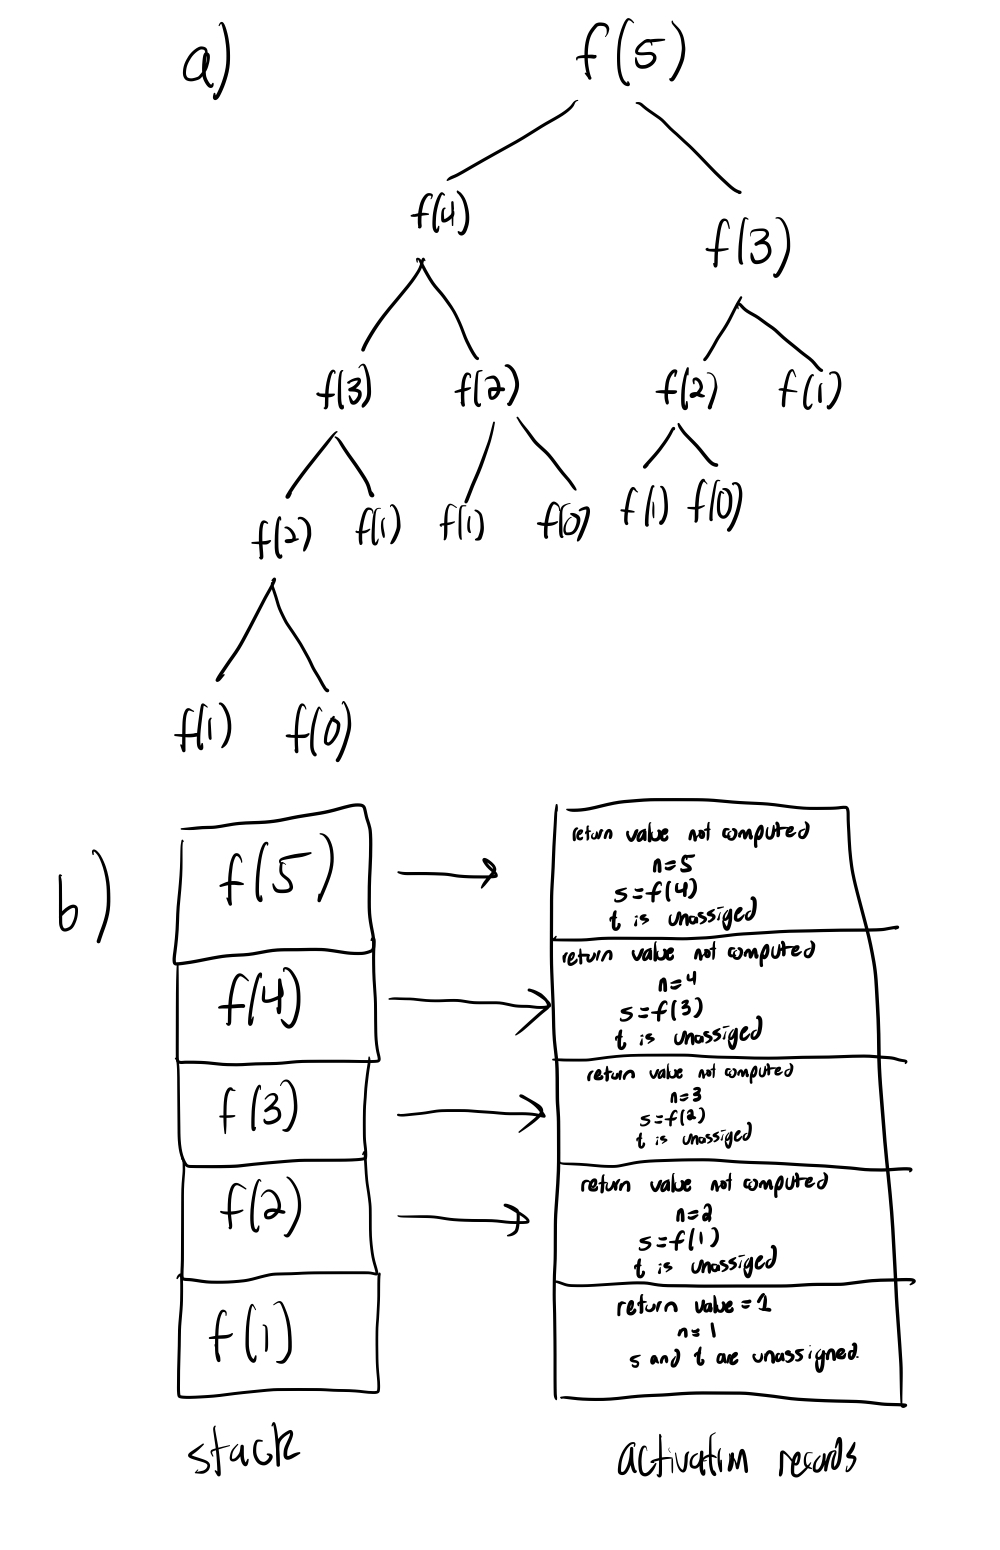
\includegraphics[scale=.4]{Prob1.jpeg}
\end{solution} 

\noindent\rule{7in}{2.8pt}

%%%%%%%%%%%%%%%%%%%%%%%%%%%%%%%%%%%%%%%%%%%%%%%%%%%%%%%%%%%%%%%%%%%%%%%%%
%%%%%%%%%%%%%%%%%%%%%%%%%%%%%%%%%%%%%%%%%%%%%%%%%%%%%%%%%%%%%%%%%%%%%%%%%
% Problem 8
%%%%%%%%%%%%%%%%%%%%%%%%%%%%%%%%%%%%%%%%%%%%%%%%%%%%%%%%%%%%%%%%%%%%%%%%%%%%%%%%%%%%%%%%%%%%%%%%%%%%%%%%%%%%%%%%%%%%%%%%%%%%%%%%%%%%%%%%

\begin{problem}{2 - 10 points}
In a language that passes parameters by reference, there is a  function $f(x;y)$ that does the following:  

$x = x + 1;\quad y = y + 2; \quad return \quad x+y;$  

\noindent If $a$ is assigned the value 3, and then $f(a;a)$ is called, what is returned? 
\end{problem}

\begin{solution}
    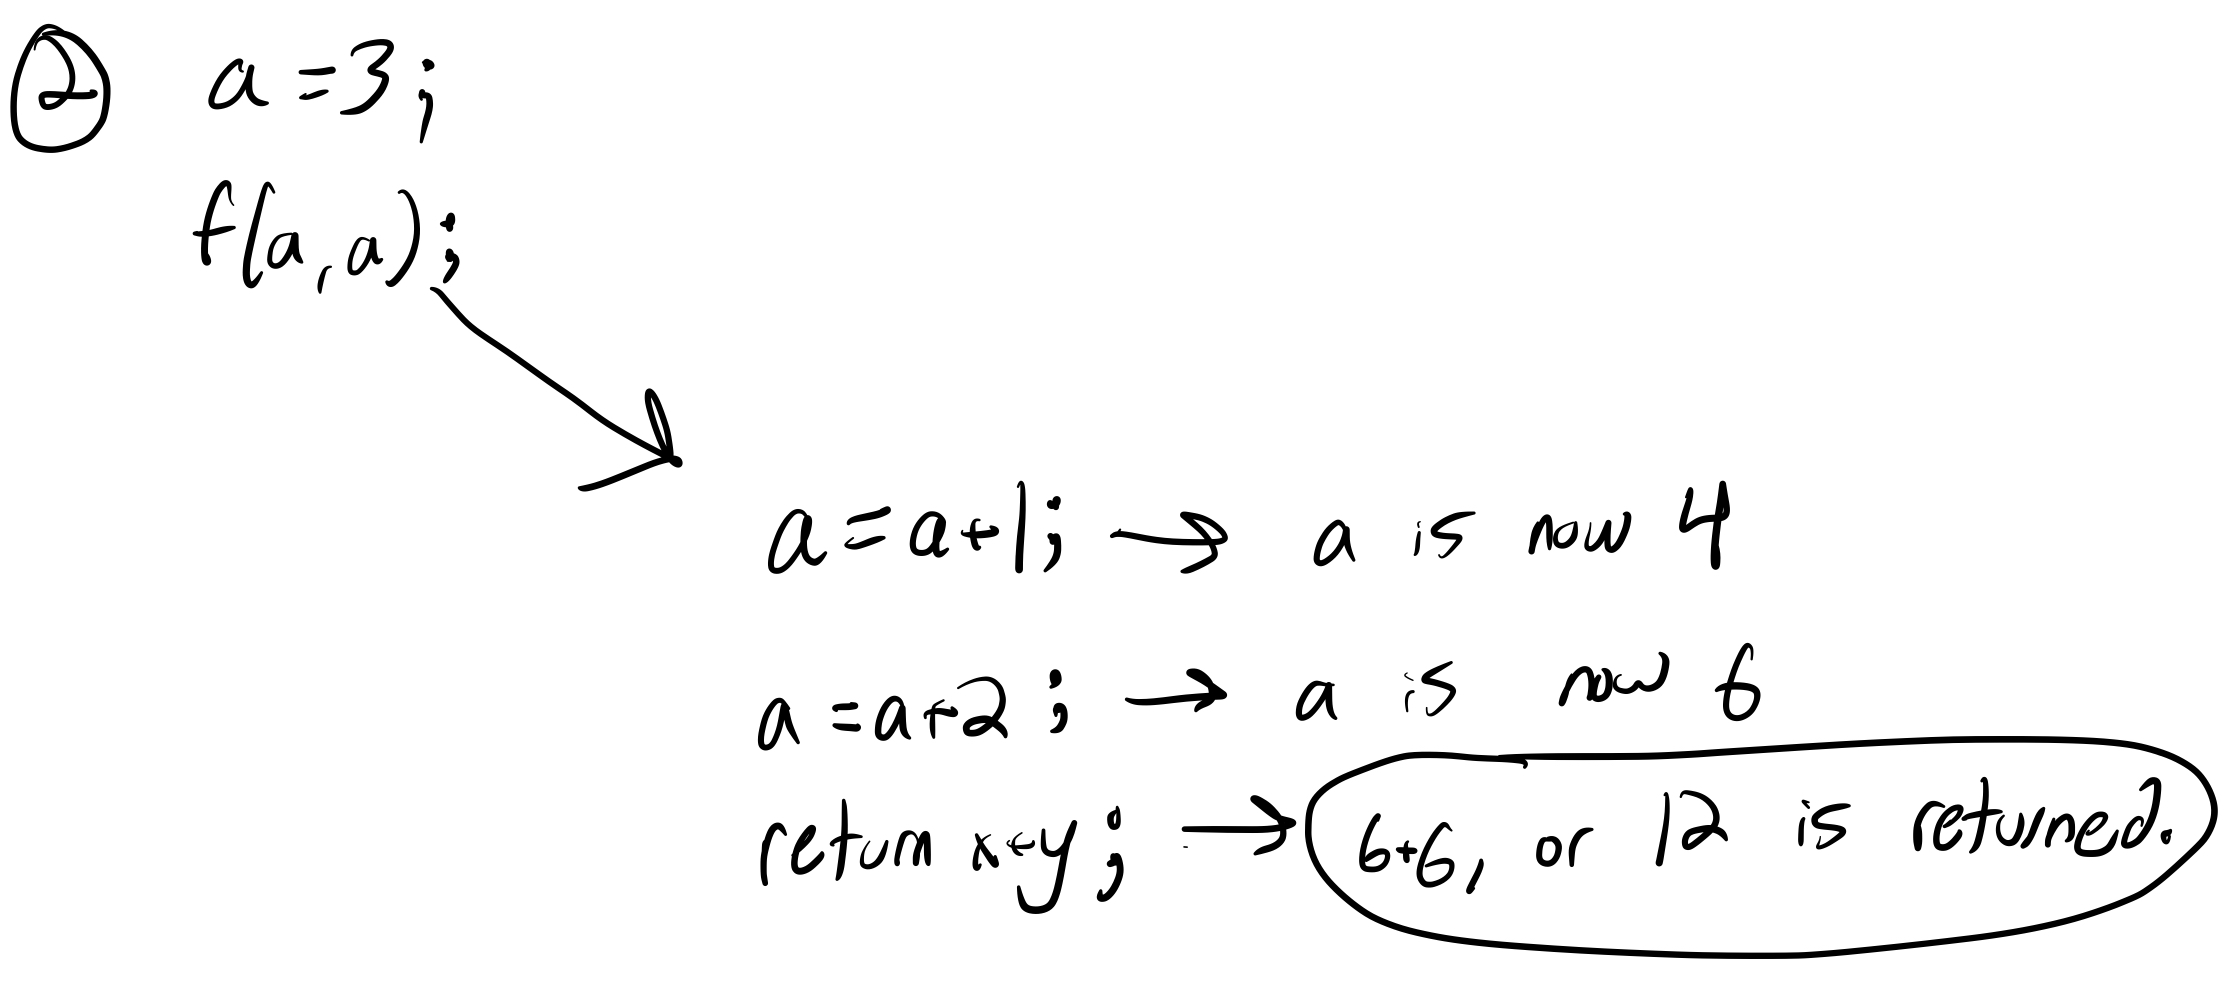
\includegraphics[scale=.2]{Prob2.jpeg}
\end{solution} 

\noindent\rule{7in}{2.8pt}

%%%%%%%%%%%%%%%%%%%%%%%%%%%%%%%%%%%%%%%%%%%%%%%%%%%%%%%%%%%%%%%%%%%%%%%%%
%%%%%%%%%%%%%%%%%%%%%%%%%%%%%%%%%%%%%%%%%%%%%%%%%%%%%%%%%%%%%%%%%%%%%%%%%
% Problem 7
%%%%%%%%%%%%%%%%%%%%%%%%%%%%%%%%%%%%%%%%%%%%%%%%%%%%%%%%%%%%%%%%%%%%%%%%%%%%%%%%%%%%%%%%%%%%%%%%%%%%%%%%%%%%%%%%%%%%%%%%%%%%%%%%%%%%%%%%

\begin{problem}{3 - 10 points}
The C function $f$ is defined by:  
\begin{verbatim}
int f(int x, *py, **ppz) {  
    **ppz += 1; *py += 2; x += 3; return x+*py+**ppz; 
} 
\end{verbatim}

\noindent Variable $a$ is a pointer to $b$ ; variable $b$ is a pointer to $c$ , and $c$ is an integer  currently with value 4. If we call $f ( c; b; a)$, what is returned? 

\end{problem}

\begin{solution}
    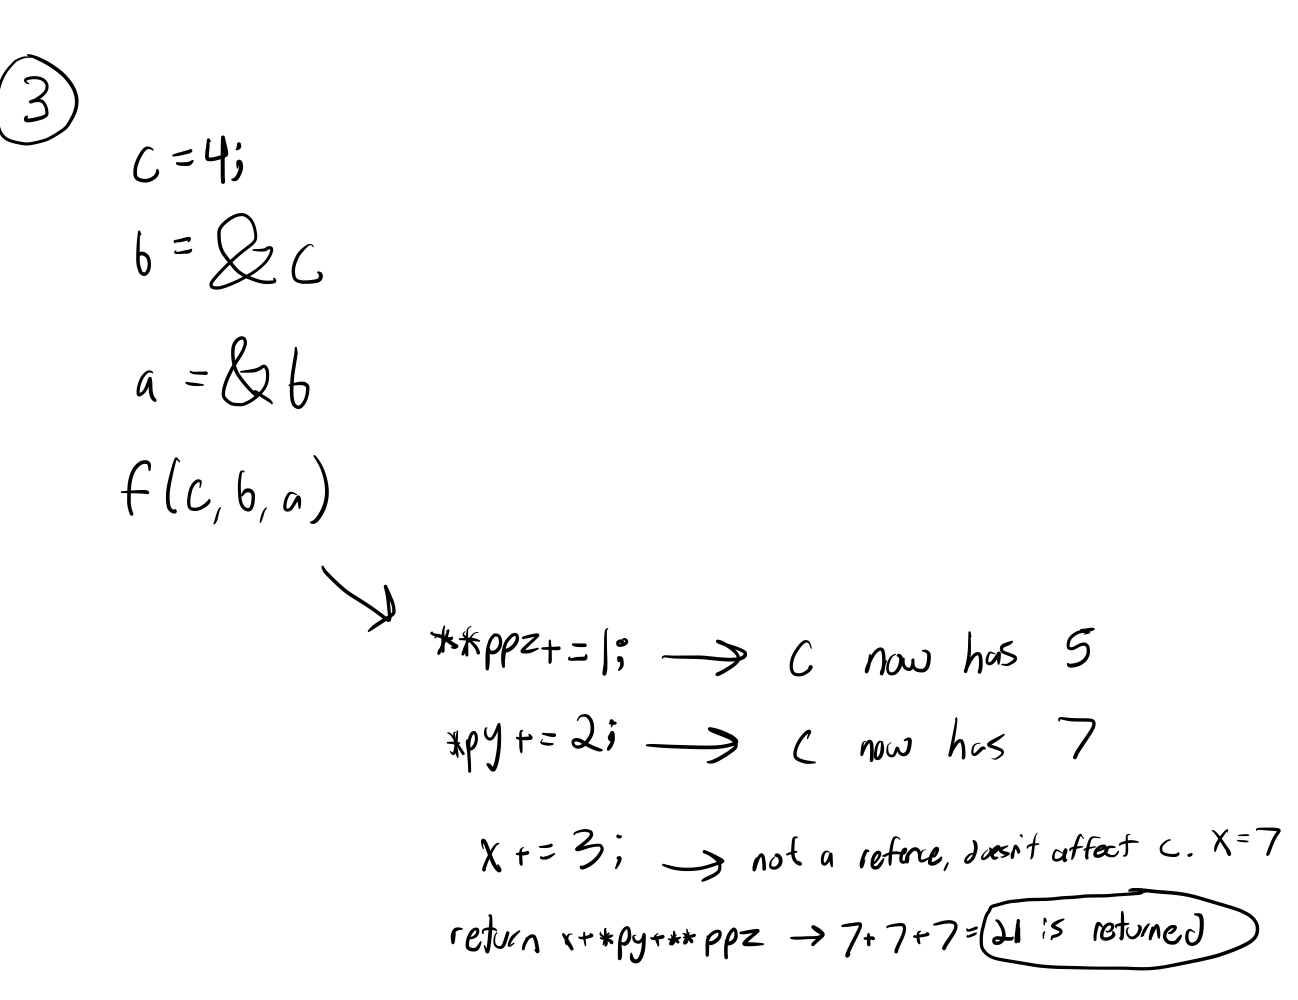
\includegraphics[scale=.3]{Prob3.jpeg}
\end{solution} 

\begin{problem}{4 - 70 points}
Write a C or C++ program to showcase some of the features of Clang and LLVM. You want to write a C program that will best showcase the features of various optimizations. Use time function inside the code to measure program time for performance measurements. Use well known algorithms (sorting, searching, numerical computation, etc.) and state where they are used if the code is more obscure.

\begin{enumerate}
    \item For a given architecture, compare the time it takes for different types of compiler optimization. Also use compiler option to minimize code size. Compare the codes (target assembly code) for all cases to isolate the types of optimizations implemented. 
    \item Show at least three different optimizations in your code that are affected by compiler optimizations. Use Transform (most important), and Utility Passes  (https://llvm.org/docs/Passes.html) that are applicable to your example with complete makefile (or command line script) for the passes and appropriate documentation of results. You may also want to refer to clang.llvm.org
    
\end{enumerate}

\end{problem}
\noindent\rule{7in}{2.8pt}
%%%%%%%%%%%%%%%%%%%%%%%%%%%%%%%%%%%%%%%%%%%%%%%%%%%%%%%%%%%%%%%%%%%%%%%%%

%%%%%%%%%%%%%%%%%%%%%%%%%%%%%%%%%%%%%%%%%%%%%%%%%%%%%%%%%%%%%%%%%%%%%%%%%
% Problem 
%%%%%%%%%%%%%%%%%%%%%%%%%%%%%%%%%%%%%%%%%%%%%%%%%%%%%%%%%%%%%%%%%%%%%%%%%%%%%%%%%%%%%%%%%%%%%%%%%%%%%%%%%%%%%%%%%%%%%%%%%%%%%%%%%%%%%%%%

%%%%%%%%%%%%%%

%%%%%%%%%%%%%%%%%%%%%%%%%%%%%%%%%%%%%%%%%%%%%%%%%%%%%%%%%%%%%%%%%%%%%%%%%
% Deliverables
%%%%%%%%%%%%%%%%%%%%%%%%%%%%%%%%%%%%%%%%%%%%%%%%%%%%%%%%%%%%%%%%%%%%%%%%%%%%%%%%%%%%%%%%%%%%%%%%%%%%%%%%%%%%%%%%%%%%%%%%%%%%%%%%%%%%%%%%
\bf{Deliverables:} A zip file containing
\begin{itemize}
    \item File with your code
    \item README text file with directions to run the various programs
    \item Report showing original code and optimized code snippets and the particular optimization used; results (table of performance). Similarily for the bonus portion.
    \begin{itemize}
        \item Full names and Case IDs
        \item (not required) any special notes about your implementation the grader should be aware of
    \end{itemize}
    
\end{itemize}
\noindent\rule{7in}{2.8pt}

\end{document}
 